%************************************************
\chapter{Descripción de compresión JPEG con pérdida}\label{ch:jpeg_desc}
%************************************************

\section{Historia y Descripciones Breves de los Fundamentos Matemáticos}

La Teoría de Codificación es una sub-rama de la Teoría de la Información que
marcó el inicio del estudio formal de la compresión de datos. La Teoría de la
Información, nacida en 1948 con la publicación del artículo de Claude E.
Shannon ``A Mathematical Theory of Communication'' \citep{shannon}, gira
alrededor de los conceptos de \emph{densidad de información}, \emph{entropía de
información} y \emph{redundancia de información}.

La Codificación de Entropía son métodos de compresión sin pérdida de
información que no toman en cuenta el contenido. Los dos métodos más populares
actualmente son los Códigos de Huffman y la Codificación Aritmética.

Dos años después de la publicación de Shannon, David Huffman inventó lo que hoy
conocemos como Codificación Huffman \citep{Huffman}. Los Códigos de Huffman son
códigos de prefijos que minimizan la longitud de los códigos individuales. Se
mantienen hasta hoy como la técnica más aprovechada en algoritmos de compresión
sin pérdida.

Después de Huffman, el método más popular para reducir redundancia es la
Codificación Aritmética. Es un método más sofisticado que consigue mejores
resultados. Entre $5\%$ y $10\%$ según el estándar JPEG \citep{JPEGSTD}. La
especificación de la compresión JPEG incluye la capacidad de utilizar
codificación aritmética, pero en la práctica no tiende a ser usada. En
particular, las implementaciones de código abierto no podían usar legalmente
Codificación Aritmética ya que es una técnica altamente patentada
\citep{jpeg_patents}.

En 1974, Nasir Ahmed publicó un artículo describiendo su Transformada de Coseno
Discreta \emph{(DCT)}, por sus siglas en Inglés. La DCT es un caso particular
de la transformada de Fourier, restringida a los números reales.

La compresión JPEG como casi todos la usamos se basa en códigos de Huffman y en
la Transformada de Coseno Discreta.

% ============================================================
\section{Tipos de compresión}
% ============================================================

La compresión de datos puede ser \emph{con pérdida} o \emph{sin pérdida}. Una
compresión sin pérdida es una función biyectiva. El dominio de la función es el
espacio de datos que estamos interesados en comprimir. Los formatos de
compresión sin péridida funcionan identificando información redundante y
removiendo la redundancia, dejando la información intacta. La compresión con
pérdida hace esto también, pero también identifica información ``inecesaria''.
Dependiendo de la agresividad de la compresión, la pérdida de información puede
ser desde imperceptible a inaceptable.

El formato JPEG soporta varios tipos de compresión.

\begin{list}{}{} \item \emph{Baseline}

El tipo \emph{baseline} es el más popular y es el tipo de compresión en el que
se enfoca este trabajo. Por brevedad, a menos de que se especifique lo
contario, cuando el resto de este documento hable de compresión JPEG, estará
hablando del tipo \emph{baseline}. La compresión está basada en la Transformada
de Coseno Discreta para filtrar información innecesaria, y para reducir
redundancia puede utilizar Árboles de Huffman o Codificación Aritmética.

\item \emph{Progresivo}

El tipo \emph{progresivo} es similar a \emph{baseline}, pero se le agregan
propiedades deseables. La imagen se comprime en múltiples pasos, cada uno con
mayor detalle. Con el método \emph{progresivo}, se puede desplegar la imágen
sin que se tenga la totalidad de los datos en memoria.

La utilidad de este método es poder dibujar la imágen mientras se está
descargando de Internet. Cuando se está en un entorno con ancho de banda
limitado, o cuando se descarga una imágen muy grande, es de valor para el
usuario poder ver versiones de la imágen progresivamente más detalladas
mientras se descarga.

\item \emph{Sin pérdida}

La compresión sin pérdida fue agregada a JPEG ``por que tenían que'' y no hubo
un análisis riguroso para su diseño \citep{JPEGSTD}. Aunque la compresión JPEG
sin pérdida no es mala, formatos como PNG son altamente más populares y
efectivos. Mucho software simplemente no soporta JPEG con compresión sin
pérdida.

\item \emph{Compresión Jerárquica}

El modo jerárquico codifica la imágen en varias versiones, cada una a
diferentes resoluciones. Se guarda en una estructura ``piramidal''. La primera
imágen está comprimida a resolución completa, y cada imágen sucesiva se guarda
a la mitad de la resolución de la anterior. Esta pirámide se guarda en memoria
de imágen más pequeña a imágen más grande.

Este método es útil cuando la resolución de la imagen es muy grande, y la
aplicación no necesita o no es capaz de utilizar la imagen en su tamaño
completo.

\end{list}

% ============================================================
\section{Descripción de la Compresión \emph{Baseline} de JPEG}
% ============================================================

El codificador implementado en este trabajo es el \emph{Baseline JPEG}, al que
también se le refiere como \emph{DCT-Based Coding}, traducido aquí como
\emph{Codificación DCT}. Para el resto del documento, a menos que sea
necesario, se usará el término \emph{JPEG} para referirse a lo mismo que
\emph{Baseline JPEG}.

La codificación DCT divide a la imágen en bloques de $8\times8$ píxeles. Cada
bloque de $8\times8$ pasa por una serie de transformaciones y salen
secuencialmente como datos comprimidos.

El primer paso en el \emph{pipeline} es separar los componentes de la imágen.
Las dos maneras más comunes de representar imágenes en computadoras es
\verb+RGB+ o \verb+RGBA+: En ambos formatos, cada píxel ocupa 32 bits de
espacio, divididos en componentes de 8 bits. Cada componente corresponde a un
color o al valor de opacidad, comúnmente denominado \emph{alpha}. \verb+RGB+
corresponde al byte \verb+RRGGBBXX+, con \verb+RR+ representando rojo,
\verb+GG+ representando verde y \verb+BB+ representando azul. Aunque a veces
decimos que \verb+RGB+ es un formato de 24 bits, especificamos el byte
\verb+XX+ por convención, ya que siempre se utilizan 32 bits (4 bytes) para
representar RGB. \verb+RGBA+ es análogo a \verb+RGB+. Le corresponden los 4
bytes \verb+RRGGBBAA+, donde el último byte se usa para el valor \emph{alpha}.

\subsection{Endianness}

Cabe notar que diferentes plataformas tienen diferentes convenciones para
guardar colores en memoria. Windows espera que le mandemos píxeles en órden
\verb+BGRA+, ya que al inspeccionar la memoria se ve en el órden más familiar
de \verb+ARGB+ (Microsoft no ha dicho públicamente por qué reordenaron los
componentes de color pero no el de opacidad).

Este tema toca el concepto de \emph{endianness}, que es el término que usamos
para referirnos al orden de los bytes en una palabra de memoria. En
procesadores modernos, una palabra son 32 bits. 4 bytes, cada uno de 8 bits. La
mayoría de las instrucciones que se ejecutan toman palabras como parámetros, y
cuando nos importan los detalles de bajo nivel entonces debemos de entender la
diferencia entre arquitecturas \emph{little endian} y \emph{big endian}. Una
arquitectura \emph{Little endian} guarda los bytes de una palabra de izquierda
a derecha del menos significativo al más significativo. Es más claro usar el
ejemplo concreto de los colores representados en palabras de 32 bits. Un color
\verb+RGBA+ consiste de 4 bytes y en una máquina little endian se guarda en la
memoria de la computadora como \verb+ABGR+. En una máquina \emph{big endian},
se guarda de la misma manera en que lo escribirmos: \verb+RGBA+. En ambos tipos
de ordenamiento de memoria, su \emph{endianness} afecta sólamente al
ordenamiento de bytes dentro de palábras de máquina. No hay que confundirnos y
pensar que el efecto se extiende más allá de una palabra de 32 bits. Si tenemos
dos palabras \verb+U = abcd+ y \verb+V = efgh+ entonces \verb+UV+ se ve en
memoria como \verb+dcbahgfe+. Los bytes se voltean dentro de las palabras
individuales, pero las palabras siempre van de izquierda a derecha.
Procesadores ARM después de la versión 3 son \emph{bi-endian}; pueden
seleccionar su \emph{endianness} desde software.

En ensamblador con sintaxis de Intel o en el API de Windows, se utiliza
\verb+BYTE+ para denotar 8 bits, \verb+WORD+ para 16 bits, \verb+DWORD+ para 32
bits y \verb+QWORD+ para 64 bits. Esta convención viene de cuando los
procesadores eran de 16 bits, y no cambió ni en la transición a 32 bits en los
90's ni en la transición a 64 bits en los 00's

El codificador JPEG que escribimos asume que la máquina en la que se está
corriendo es \emph{little endian}.


\subsection{La DCT}

La transformada discreta de coseno, \emph{DCT} por sus siglas en Inglés, puede
representar $N$ puntos como una suma con pesos de funciones cosenoidales de
diferentes frecuencias. Es popular en compresión porque las señales que
comprimimos tienden a tener una representación con bajas frecuencias
predominantes. Por ejemplo, es más común una imagen de un cielo azul que ruido
blanco en todos los colores. Una imagen de un cielo azul tiene muy poca
variación, que al aplicar \emph{DCT} resulta en un peso alto para frecuencias
bajas y pesos más cercanos a cero para frecuencias más altas.

En JPEG, se divide la imagen en bloques de $8\times8$ y se utiliza una \emph{DCT} de $8\times8$:
\begin{equation}\label{eq:dct}
F(u, v) = \frac{1}{4} C(u)C(v) \sum_{x=0}^{7}\sum_{y=0}^{7}
f(x,y)*\cos{\frac{(2x+1)u\pi}{16}}\cos{\frac{(2y+1)v\pi}{16}}
\end{equation}
donde \[C(u), C(v) = \begin{cases}
        \frac{1}{\sqrt{2}} & \quad \text{para } u,v = 0\\
        1                  & \quad \text{para } u,v \neq 0\\
\end{cases} \]
\begin{eqnarray*}
    f(u, v) \text{ es un punto del bloque de } 8\times8 \text{ de la imagen }\\
    F(u, v) \text{ es la DCT para el punto } u,v\\
\end{eqnarray*}

De la ecuación \ref{eq:dct} se puede derivar directamente un algoritmo para la
\emph{DCT}:

\label{alg:dct}
\begin{code}[language=C][h]
    float DCT[64];
    for (int v = 0; v < 8; ++v) {
        for (int u = 0; u < 8; ++u) {
            DCT[v*8 + u] = F(u, v);
            // F es la traducción directa de definición DCT
    }
\end{code}


La implementación de JPEG que escribí se llama \verb+tiny_jpeg+
\citep{tiny_jpeg} y contiene dos implementaciones de \emph{DCT}, la que se
muestra arriba, y una más rápida, desarrollada por \citep{ahmed_dct}.

Los algoritmos rápidos para calcular la \emph{DCT} están basados en la
observación de que la ecuación \ref{eq:dct} es lineal, y por lo tanto el
cálculo \emph{DCT} se puede ver como una multiplicación de dos matrices de
$8\times8$. La matriz de la derecha es el bloque con los valores de la imagen y
la matriz de la izquierda es la representación como matriz de la ecuación
\ref{eq:dct}.

\subsection{YUV}\label{sub:yuv}

Para generar los bloques que van a ser procesados por \emph{DCT}, la imagen se separa en tres componentes. JPEG no usa el espacio de color \verb+RGB+, usa \verb+YUV+, también denominado \verb+YCrCb+

\begin{figure}
    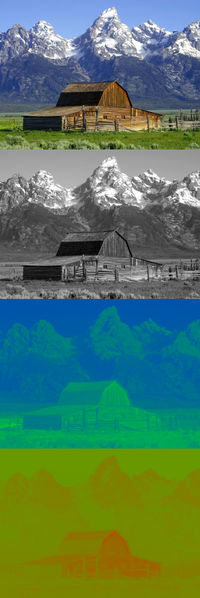
\includegraphics{yuv}
    \caption{Descomposición de una imagen a un canal de Luma y dos de Chroma}
\end{figure}


\verb+Y+ corresponde a Luminancia o Luma


\begin{figure}[hb] % h quiere decir "here". Queremos mostrar la imagen despues de explicar lo que es...
    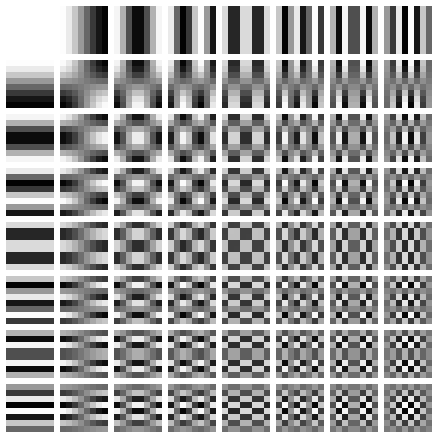
\includegraphics{DCT-8x8}
    \caption{Visualización de las funciones para el DCT de 8x8 usado en JPEG. Esquina superior izquierda: menor frecuencia. Inferior derecha: mayor frecuencia.}
\end{figure}

%%% Local Variables:
%%% mode: latex
%%% ispell-local-dictionary: "espanol"
%%% TeX-engine: xelatex
%%% TeX-master: "../tesis"
%
